\documentclass{beamer}

%
% Choose how your presentation looks.
%
% For more themes, color themes and font themes, see:
% http://deic.uab.es/~iblanes/beamer_gallery/index_by_theme.html
%
\mode<presentation>
{
  \usetheme{Warsaw}      % or try Darmstadt, Madrid, Warsaw, ...
  \usecolortheme{crane} % or try albatross, beaver, crane, ...
  \usefonttheme{structurebold}  % or try serif, structurebold, ...
  \setbeamertemplate{navigation symbols}{}
  \setbeamertemplate{caption}[numbered]
} 

\addtobeamertemplate{navigation symbols}{}{%
    \usebeamerfont{footline}%
    \usebeamercolor[fg]{footline}%
    \hspace{2em}%
    \insertframenumber/\inserttotalframenumber
}

\setbeamercolor{footline}{fg=black}
\setbeamerfont{footline}{series=\bfseries}


\usepackage[english]{babel}
\usepackage[utf8]{inputenc}
\usepackage[T1]{fontenc}
\usepackage{float}
\usepackage[caption = false]{subfig}


\title[Isospectralization]{Isospectralization, or how to hear shape, style, and correspondence}
\author{Sricharan Chiruvolu}

\institute{Zorah Lähner}
\date{\today}


\begin{document}

\begin{frame}
  \titlepage
\end{frame}

% Uncomment these lines for an automatically generated outline.
% \begin{frame}{Outline}
%  \tableofcontents
% \end{frame}

% ● ~20 slides
% ● use visualizations
% ● number your slides
% ● do not make slides full of text
% ● explain things you had problems
% understanding when first reading your
% paper in more detail
% ● reference the original authors
% Recommended structure
% 1. Introduction of the problem
% 2. Approach
% 3. Results (if any)
% 4. Summary



\section{Introduction}

\begin{frame}{Introduction}

\begin{itemize}
  \item Published in CVPR 2019.
  \item Explores the \texttt{practical} possibility of using the spectrum of an object for shape reconstruction.
  \item Proposes an inverse mapping between geometric domain and its Laplacian via simple \texttt{regularizers}.
  \item \texttt{Isospectralization}: A numerical optimization procedure to deform a mesh in order to align its (finite) Laplacian spectrum with a given one.
\end{itemize}

\end{frame}

\begin{frame}{Isospectralization}

\begin{figure}
    \centering
    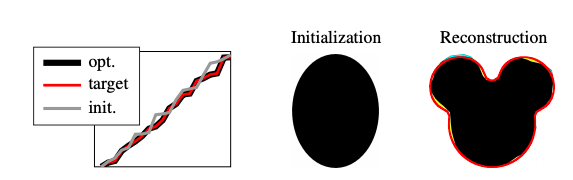
\includegraphics[height=0.2\textwidth]{Spectral.png}
    \caption{Isospectralization}
    \label{fig:Isospectralization}
\end{figure}


\end{frame}



\section{Background: Spectral Geometry}


\begin{frame}{Spectral Geometry}

\begin{itemize}
  \item Relationship between geometric structures of manifolds and spectra of canonically defined differential operators.
  \item Eigenvalue problems involving the Laplace operator on manifolds have proven to be a consistently fertile area of geometric analysis with deep connections to number theory, physics, and applied mathematics. 
\end{itemize}

\end{frame}

\subsection{Riemannian Manifold and Geodesics}

\begin{frame}{Manifolds}

(As discussed in previous talks) In computer vision, the notion of a manifold is used quite frequently.

\begin{itemize}
  \item in rotation averaging (SO3),
  \item structure and motion (“Essential” manifold)
  \item to capture the shape of an object (“Shape” manifolds)
  \item to model a set of images (“Grassman” manifolds)
  \item to simply represent a sphere ($S^n$).
  \item ...
\end{itemize}

\end{frame}

\begin{frame}{Riemannian Manifold and Geodesics}
(As discussed in previous talks)
\begin{itemize}
\item A \texttt{Riemannian} manifold is a manifold with an inner product defined in the tangent space at each point.

% TODO: remove metrics and just give idea. Talk in relation with the surface and laplace
% \item A \texttt{Riemannian} metric (tensor) makes it possible to define several geometric notions on a Riemannian manifold, such as angle at an intersection, length of a curve, area of a surface and higher-dimensional analogues (volume, etc.), extrinsic curvature of sub-manifolds, and intrinsic curvature of the manifold itself.

\item \texttt{Geodesics} are locally shortest curves. They preserve a direction on a surface and have many interesting properties.
\end{itemize}

\end{frame}

\begin{frame}{Riemannian Manifold and Geodesics}

\begin{figure}
 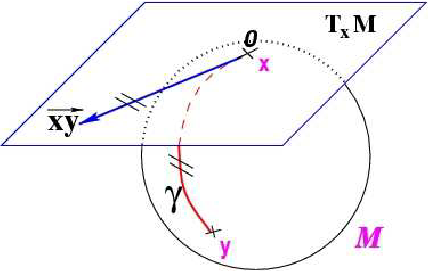
\includegraphics[height=0.3\textwidth]{Geodesics2.png}
 \caption{\label{fig:Geodesics}Geodesic and tangent space in a Riemannian manifold. \footnote{Medinria: DT-MRI processing and visualization software; Xavier Pennec.}}
\end{figure}

\end{frame}


\subsection{Isometry and Isomorphism}


\begin{frame}{Isometry and Isomorphism}

% TODO: Less text, try to get an image here. Talk about "sameness". from Functional Maps paper.
%   \item \texttt{Isometry} of a manifold can be defined in simpler terms as any (smooth) mapping of that manifold (into itself, or into another manifold) that preserves the notion of distance between points.
%   \item When such a mapping is on smooth manifolds (and is a diffeomorphism: the mapping is a bijection and its inverse is differentiable), it is called isometry, and provides a notion of \texttt{isomorphism} (“sameness”).

\begin{figure}
    \centering
    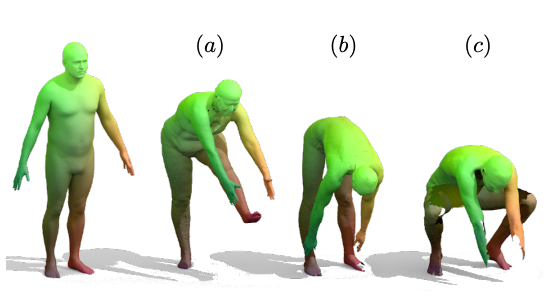
\includegraphics[height=0.4\textwidth]{isometry.png}
    \caption{Isometry and Isomorphism.\footnote{Smooth Shells: Multi-Scale Shape Registration with Functional Maps; Eisenberger, Lahner and Cremers.}}
    \label{fig:my_label}
\end{figure}

\end{frame}

% \begin{frame}{Isometry and Isomorphism}

% % maybe remeove it

% Definition : A local isometry between two Riemannian manifolds $ M $ and $ N $ is a local diffeomorphism $ h: M \rightarrow  N $, such that, for all points $ x \in M $ and all vectors $ v $ and $ w $ in $ T_{x}M $,

% $$ <v, w> = <(Dh){x}(v), (Dh){x}(w)> $$


% \end{frame}


\subsection{Laplace-Beltrami Operator}

\begin{frame}{Laplace-Beltrami Operator}

% \begin{figure}
% \subfloat[fig 1]{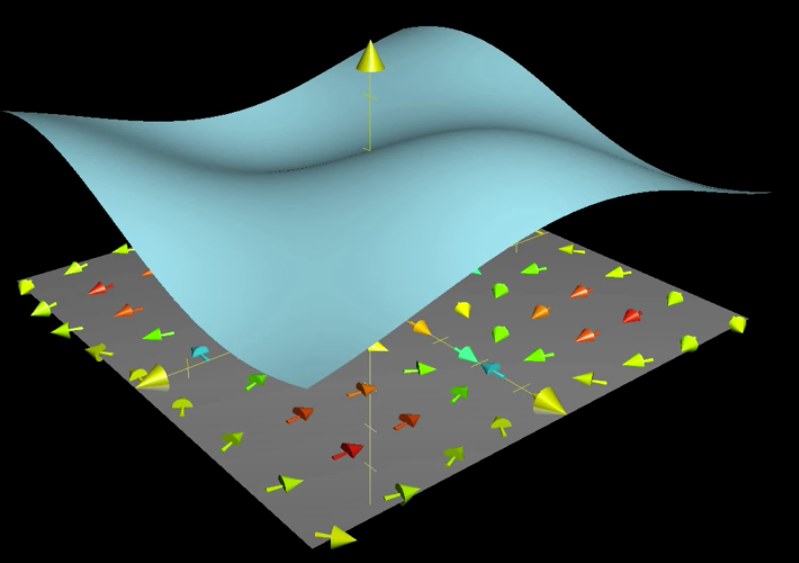
\includegraphics[width = 0.2\textwidth]{laplacian.png}} 
% \subfloat[fig 2]{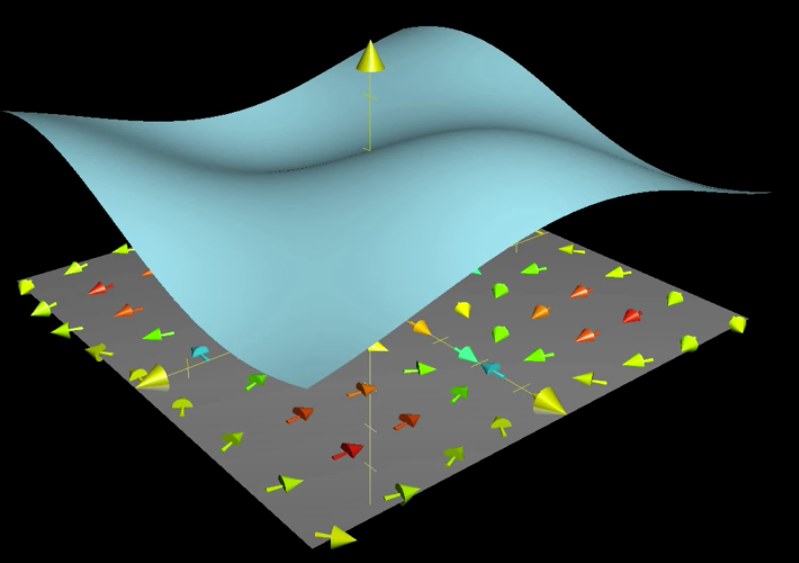
\includegraphics[width = 0.2\textwidth]{laplacian.png}}\\
% \caption{Add your own figures before compiling}
% \label{some example}
% \end{figure}

\begin{figure}
    \centering
    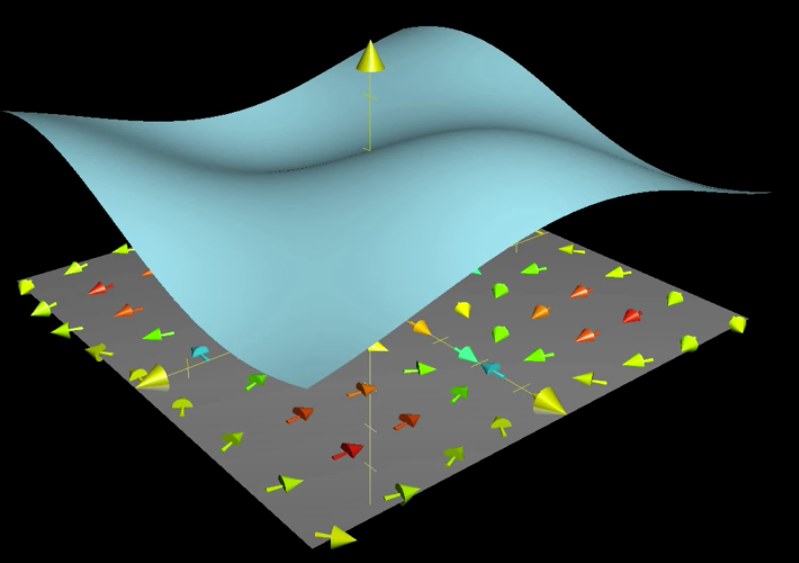
\includegraphics[width=0.4\textwidth]{laplacian.png}
    \caption{Laplace-Beltrami operator \footnote{Khan Academy; Grant Sanderson.}}
    \label{fig:laplacian}
\end{figure}

\begin{itemize}
% add divg of gradient
% explain the Laplacian from the 3b1b video.
  \item Laplacian ($ {\triangle} f $) = div(gradient($f$)).
  \item The Laplacian is generalized to the Riemannian manifold $ (M;g) $ by the Laplace-Beltrami operator ($ {\triangle}_g $).
\end{itemize}

\end{frame}

\subsection{Direct and Inverse Problems}

\begin{frame}{Isospectrals}
% Say that spectrum is the eigenvaliues
\begin{itemize}
  \item Given a compact Riemannian manifold, we can associate to it the Laplace-Beltrami operator.
  
  \item Two closed Riemannian manifolds are said to be \texttt{isospectral} if the eigenvalues of their Laplace–Beltrami operator (Laplacians) coincide.

\item Thus, \texttt{spectral geometry} is the connection between the spectrum $ Spec(M; g)$, i.e. the eigenvalues, and the geometry of the manifold $ (M; g) $. 

\item This fundamentally deals with two kinds of problems:
    \begin{itemize}
        \item Direct problems
        \item Inverse problems
    \end{itemize}

\end{itemize}

\end{frame}

\begin{frame}{Direct and Inverse Problems}

\begin{block}{Direct Problems}

    Direct problems attempt to infer the behavior of the eigenvalues of a Riemannian manifold from knowledge of the geometry.

\textit{Compute (exactly or not) the spectrum $ Spec(M, g) $? And (or) find properties on the spectrum $ Spec(M,g) $?}

\end{block}

\begin{block}{Inverse Problems}
     
     Inverse problem - does the data of the spectrum $ Spec(M, g) $ determine the "shape" of the manifold $ (M, g) $ ?

\textit{Which geometric information of the manifold can we determine from the spectrum?}
\end{block}

\end{frame}

\section{Approach: Isospectralization}

\subsection{Hearing the Shape of a Drum}

\begin{frame}{Hearing the Shape of a Drum}

\begin{figure}
    \centering
    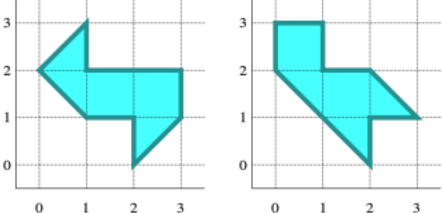
\includegraphics[height=0.2\textwidth]{Indenticalshapes.png}
    \caption{Membranes of these two different shapes (but otherwise identical) would "sound" the same.}
    \label{fig:Identicalshapes}
\end{figure}

\begin{block} {"Can one hear the shape of a drum?"}
    Mark Kac's 1966 question, "Can one hear the shape of a drum?" set off research into spectral theory, with the idea of understanding the extent to which the spectrum allows one to read back the geometry. 
\end{block}


\end{frame}

\begin{frame}{Hearing the Shape of a Drum}

\begin{itemize}
% TODO: one slide per idea.
    \item Theoretically Negative. \texttt{Why?} - There exists isospectral manifolds that are nonisometric.
    \item With additional priors, practically feasible. We can recover the structure of an object from its spectrum.
    
\end{itemize}
    
\end{frame}

% \begin{frame}{Applications}

% \begin{itemize}
%     \item \texttt{Finding Intrinsic Coordinates} - Can be used as a universal pre-processing technique for general correspondence matching problems.
%     \item  \texttt{Non-isometric Shape Matching} - Can be used to find correspondences between non-rigid shapes (intrinsic isometrics).
%     \item  \texttt{Style/ Pose Transfer}.
    
% \end{itemize}
    
% \end{frame}


\subsection{Isospectralization}

\begin{frame}{Notations}
\begin{figure}
 \includegraphics[width=\textwidth]{notations}
 \caption{\label{fig:notations}Notations}
\end{figure}
\begin{itemize}
    \item Discretization.
\end{itemize}
\end{frame}

\begin{frame}{Isospectralization}

\textbf{Find the optimal embedding that aligns the spectrum to another:}

 $$ \min _{\mathbf{V} \in \mathbb{R}^{n \times d}}\left\|\boldsymbol{\lambda}\left(\boldsymbol{\Delta}_{X}(\mathbf{V})\right)-\boldsymbol{\mu}\right\|_{\omega}+\rho_{X}(\mathbf{V}) $$

\vskip 0.5cm

    \begin{itemize}
        \item $\mathbf{V}$ is the (unknown) embedding of the mesh vertices in $\mathbb{R}$.
        \item $\boldsymbol{\Delta}_{X}(\mathbf{V})$ is the associated discrete Laplacian.
        % \item $\rho_{X}(\mathbf{V})$ is a regularizer for the embedding, implementing the natural expectation that the sought solution should satisfy certain desirable properties.
        % \item Assumption: Knowledge of limited portion of the spectrum is enough to fix the shape of the domain, given some minimal amount of additional information - \texttt{Regularizers}.
    \end{itemize}
    
\end{frame}


\subsection{Regularizers for flat shapes}

\begin{frame}{Flat Shape Regularizers}

\begin{itemize}
    \item Encourage Smaller Boundary Edge Lengths
    
    $$ \rho_{X}(\mathbf{V}) = \sum_{e_{ij} \in E_{b}} l_{ij}(\mathbf{V}) $$
    
    \item Penalize Triangle Flips
    
    $$\rho_{X}(V)=\left(\min \left(0, r_{X}(V)\right)\right)^{2}$$
    
   $$r_{X}(V)=\sum_{i j k \in F}\left(R \pi / 2_{2}\left(\mathbf{v}^{j}-\mathbf{v}^{i}\right)\right)^{T}\left(\mathbf{v}^{k}-\mathbf{v}^{i}\right)$$

    
\end{itemize}
    
\end{frame}

\begin{frame}{Flat Shape Regularizers}

\begin{itemize}

    \item Encourage Small Interior Edge Lengths
    
    $$ \rho_{X}(\mathbf{V}) = \sum_{e_{ij} \in E_{i}} l_{ij}^2(\mathbf{V}) $$
    
    \item Note: Optimization is effected by the mesh resolution and spectral bandwidth.
    
\end{itemize}
    
\end{frame}

\begin{frame}{Shape reconstruction on Flat Shapes}

\begin{figure}
 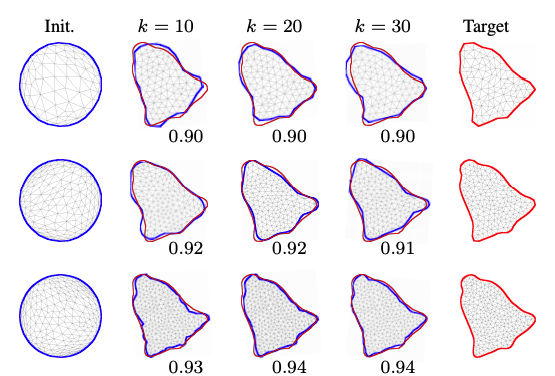
\includegraphics[height=0.5\textwidth,keepaspectratio]{Flatshapes}
 \caption{\label{fig:Flatshapes} Shape recovery optimization for flat shapes.}
\end{figure}
    
\end{frame}


\subsection{Regularizers for surfaces shapes}

\begin{frame}{Surface Regularizers}

\begin{itemize}
    \item Encourage Vertices to Lie Close to Barycenter of neighbors, $ \mathbf{L} $ is the initial graph Laplacian.
    
    $$ \rho_{X}(\mathbf{V}) = \left\| \mathbf{L}_0^g \mathbf{V}  \right\|_{2}^{2} $$
    
    \item Encourage small total displacement from initial embedding - volume to grow/shrink to disambiguate isometric shapes.
    
    $$ \rho_{X}(\mathbf{V})=\sum_{i=1}^{n}\left(a_{i}\left(\mathbf{v}^{i}-\mathbf{v}_{0}^{i}\right)\right)^{2} $$
    
\end{itemize}
    
\end{frame}

\begin{frame}{Shape reconstruction on Surfaces}
% TODO: Regularizer is an arbituary choice the result 1 isn't technically wrong. 
\begin{figure}
 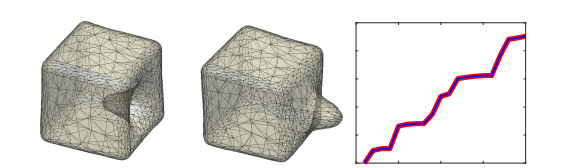
\includegraphics[width=\textwidth]{Surfaces}
 \caption{\label{fig:Surfaces} Two isometric shapes ("Surfaces") with different volume; their (identical) spectra. This is the reason we need the second Regularizer.}
\end{figure}
    
\end{frame}

% \begin{frame}{Shape reconstruction on Surfaces}

% \begin{figure}
%     \centering
%     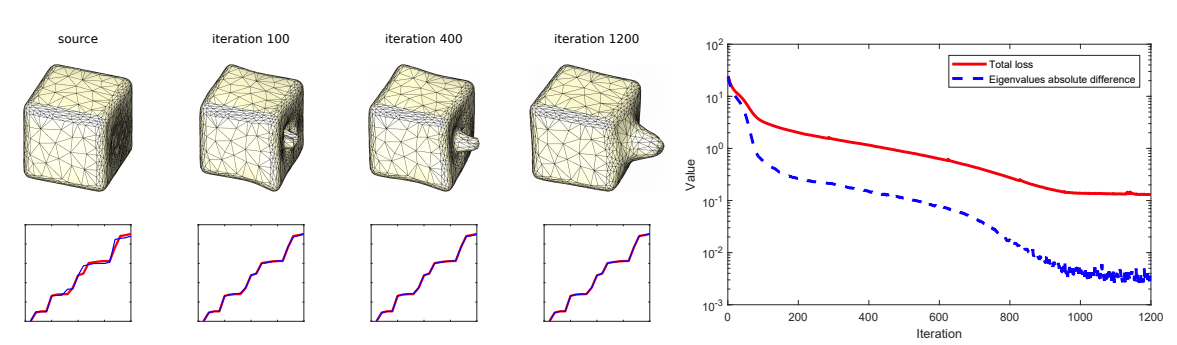
\includegraphics[width=\textwidth]{Surfaces2.png}
%     \caption{Shape reconstruction on Surfaces}
%     \label{fig:abel}
% \end{figure}
    
% \end{frame}

\section{Applications/Results}


\subsection{Non-isometric shape matching}

\begin{frame}{Non-isometric shape matching}
    
\begin{figure}
 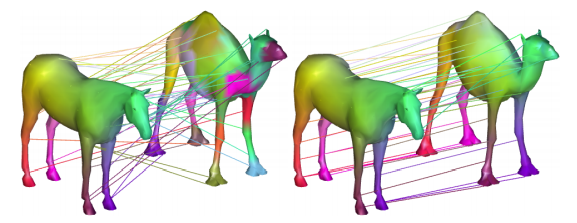
\includegraphics[width=\textwidth]{Correspondenses.png}
 \caption{\label{fig:Correspondenses} Isospectralization as pre-processing for dense correspondence matching.}
\end{figure}
    
    
\end{frame}


% \begin{frame}{Non-isometric shape matching}
    
% \begin{figure}
%  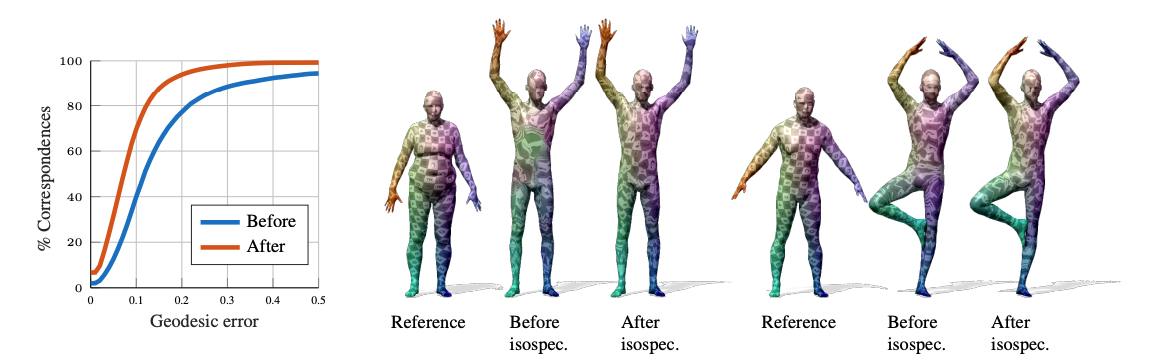
\includegraphics[width=\textwidth]{FAUST.png}
%  \caption{\label{fig:FAUST} Non-isometric shape matching on FAUST dataset. Texture maps to Correspondences.}
% \end{figure}
    
    
% \end{frame}




\subsection{Style Transfer}

\begin{frame}{Style Transfer}
% Different inits (in this case the poses) gives different results.
\begin{figure}
    \centering
    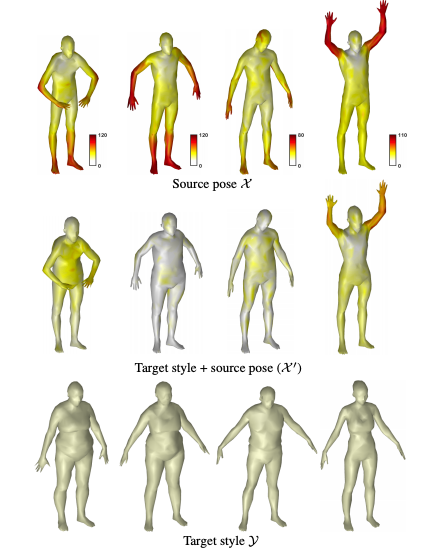
\includegraphics[height=0.5\textwidth]{Styletransfer.png}
    \caption{Isospectralization for Style Transfer}
    \label{fig:styletransfer}
\end{figure}
    
\end{frame}


\section{Summary}

\begin{frame}{Summary}
    \begin{itemize}
        \item Improvement for modern shape matching problems via addressing a decades-old problem. 
        \item Applications in various domains of geometry processing and computer vision.
        \item No mathematical backing on optimization yet.
        \item No experimental proof on shape interpolation yet.
    \end{itemize}
\end{frame}


\begin{frame}{End}
    \begin{itemize}
        \item Quick Demo.
        \item Questions.
        \item Thanks for listening!
    \end{itemize}
\end{frame}






% \section{Introduction}

% \begin{frame}{Introduction}

% \begin{itemize}
%   \item Your introduction goes here!
%   \item Use \texttt{itemize} to organize your main points.
% \end{itemize}

% \vskip 1cm

% \begin{block}{Examples}
% Some examples of commonly used commands and features are included, to help you get started.
% \end{block}

% \end{frame}


% \section{Some \LaTeX{} Examples}

% \subsection{Tables and Figures}

% \begin{frame}{Tables and Figures}

% \begin{itemize}
% \item Use \texttt{tabular} for basic tables --- see Table~\ref{tab:widgets}, for example.
% \item You can upload a figure (JPEG, PNG or PDF) using the files menu. 
% \item To include it in your document, use the \texttt{includegraphics} command (see the comment below in the source code).
% \end{itemize}

% % Commands to include a figure:
% %\begin{figure}
% %\includegraphics[width=\textwidth]{your-figure's-file-name}
% %\caption{\label{fig:your-figure}Caption goes here.}
% %\end{figure}

% \begin{table}
% \centering
% \begin{tabular}{l|r}
% Item & Quantity \\\hline
% Widgets & 42 \\
% Gadgets & 13
% \end{tabular}
% \caption{\label{tab:widgets}An example table.}
% \end{table}

% \end{frame}

% \subsection{Mathematics}

% \begin{frame}{Readable Mathematics}

% Let $X_1, X_2, \ldots, X_n$ be a sequence of independent and identically distributed random variables with $\text{E}[X_i] = \mu$ and $\text{Var}[X_i] = \sigma^2 < \infty$, and let
% \[ S_n = \frac{X_1 + X_2 + \cdots + X_n}{n}
%       = \frac{1}{n}\sum_{i}^{n} X_i \]
% denote their mean. Then as $n$ approaches infinity, the random variables $\sqrt{n}(S_n - \mu)$ converge in distribution to a normal $\mathcal{N}(0, \sigma^2)$.

% \end{frame}

\end{document}